\chapter{Расчет параметров выпрямительной установки возбуждения (ВУВ)}
\section{Определение эксплуатационных характеристик ВУВ}

В качестве ВУВ используем однофазный управляемый двуполупериодный выпрямитель, выполненный по мостовой схеме. При сборе схемы электродинамического торможения, обмотки возбуждения всех тяговых двигателей секции электровоза соединяются последовательно и подключаются к выходу ВУВ. 

Расчетная схема силовой части ВУВ изображена на рисунке~\ref{fig:vuv}.

\begin{figure}[H]
    \centering    
    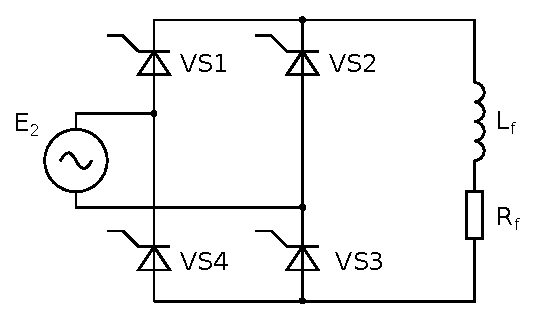
\includegraphics[width=0.5\textheight]{rectifier.eps}
    \caption{Расчетная схема силовой части выпрямительной установки возбуждения: $E_2$ - ЭДС обмотки тягового трансформатора, выделенной для питания ВУВ; VS1~--~VS4 - однооперационные тиристорные ключи; $L_f, \, R_f$ - соответственно, эквивалентная индуктивность и эквивалентное активное сопротивление обмоток возбуждения ТЭД.}
    \label{fig:vuv}
\end{figure}
